\documentclass{article}
\usepackage[utf8]{inputenc}
\usepackage{graphicx}
\usepackage{wrapfig}
\usepackage{listings}
\usepackage[margin=48pt]{geometry}
\usepackage{fancyhdr}
\pagestyle{fancy}
\fancyhead{}

\chead{Método de Muller}

\title{\textbf{Método de Muller}}
\author{Juan David Páez Sánchez \\Ingeniería de Sistemas\\ jd.paez@javeriana.edu.co \and Santiago Zúñiga Martinez\\ Ingeniería de Sistemas\\ s.zunigam@javeriana.edu.co}
\date{Pontificia Universidad Javeriana\\FECHA DE ENTREGA}

\begin{document}

\maketitle

\section{Introducción}
A la hora de solucionar ecuaciones no lineales en una variable, 
es decir encontrar o aproximar sus raíces, se pueden utilizar 
distintos métodos, como el despeje directamente, Newton, posición falsa, 
entre otros. Sin embargo, se presenta un problema cuando las funciones que 
queramos evaluar tengan raíces complejas, ya que los métodos mencionados 
anteriormente no son los indicados para este tipo planteamientos. 
Es por eso que el matemático estadounidense, David Eugene \textbf{Muller}, 
propuso un método para poder obtener un aproximación de este tipo de 
funciones el cual será explicado y desarrollado a lo largo de este documento.
\
\section{Definición}
El método de Muller, esta muy relacionado con el método de la secante, 
teniendo en cuenta que este consiste en tener una aproximación de la 
raíz a partir de dos puntos en la función $F(x)$. En el caso de 
Muller consiste en tener 3 puntos sobre la gráfica de la función, 
siendo estos una composición cuadrática, la cual da una aproximación de la raíz compleja de $F(x)$.
\begin{figure}[h]
    \centering
        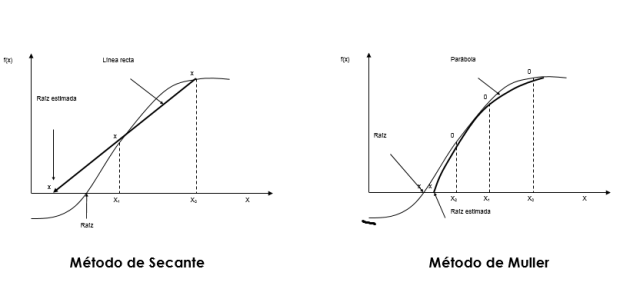
\includegraphics[scale=0.6]{Imagenes/MetodoSecanteYMuller.png}
        \caption{ESTO SE VA A BORRAR ES PARA PROBAR LAS IMAGENES}
    \label{fig:1}
\end{figure}
\end{document}
